%% Template para dissertação/tese na classe UFPEthesis
%% versão 0.9.2
%% (c) 2005 Paulo G. S. Fonseca
%% www.cin.ufpe.br/~paguso/ufpethesis

%% Carrega a classe ufpethesis
%% Opções: * Idiomas
%%           pt   - português (padrão)
%%           en   - inglês
%%         * Tipo do Texto
%%           bsc  - para monografias de graduação
%%           msc  - para dissertações de mestrado (padrão)
%%           qual - exame de qualificação doutorado
%%           prop - proposta de tese doutorado
%%           phd  - para teses de doutorado
%%         * Mídia
%%           scr  - para versão eletrônica (PDF) / consulte o guia do usuario
%%         * Estilo
%%           classic - estilo original à la TAOCP (deprecated)
%%           std     - novo estilo à la CUP (padrão)
%%         * Paginação
%%           oneside - para impressão em face única
%%           twoside - para impressão em frente e verso (padrão)
\documentclass[oneside, bsc]{ufpethesis}

%% Preâmbulo:
%% coloque aqui o seu preâmbulo LaTeX, i.e., declaração de pacotes,
%% (re)definições de macros, medidas, etc.
%!TEX root = ./main.tex
\usepackage{tikz}
\usetikzlibrary{decorations.pathmorphing,patterns}
\usepackage{pgfplots}
\pgfplotsset{compat=1.8}

\usepackage{units}

\newcommand{\norm}[1]{\lVert#1\rVert}

\newcommand*{\vv}[1]{\overrightarrow{#1}}
%% Identificação:

% Universidade
% e.g. \university{Universidade de Campinas}
% Na UFPE, comente a linha a seguir
\university{Universidade Federal de Pernambuco}

% Endereço (cidade)
% e.g. \address{Campinas}
% Na UFPE, comente a linha a seguir
\address{Recife}

% Instituto ou Centro Acadêmico
% e.g. \institute{Centro de Ciências Exatas e da Natureza}
% Comente se não se aplicar
\institute{Centro de Informática}

% Departamento acadêmico
% e.g. \department{Departamento de Informática}
% Comente se não se aplicar
% \department{<NOME DO DEPARTAMENTO>}

% Programa de pós-graduação
% e.g. \program{Pós-graduação em Ciência da Computação}
\program{Graduação em Ciência da Computação}

% Área de titulação
% e.g. \majorfield{Ciência da Computação}
\majorfield{Ciência da Computação}

% Título da dissertação/tese
% e.g. \title{Sobre a conjectura $P=NP$}
\title{Síntese de Áudio Realístico com Modelagem Física: Acelerando a computação da Radiação Acústica em GPU}

% Data da defesa
% e.g. \date{19 de fevereiro de 2003}
\date{19 de Julho de 2016}

% Autor
% e.g. \author{José da Silva}
\author{Rafael Farias Marinheiro}

% Orientador(a)
% Opção: [f] - para orientador do sexo feminino
% e.g. \adviser[f]{Profa. Dra. Maria Santos}
\adviser{Geber Lisboa Ramalho}

% Orientador(a)
% Opção: [f] - para orientador do sexo feminino
% e.g. \coadviser{Prof. Dr. Pedro Pedreira}
% Comente se não se aplicar
% \coadviser{NOME DO(DA) CO-ORIENTADOR(A)}

%% Inicio do documento
\begin{document}

%%
%% Parte pré-textual
%%
\frontmatter

% Folha de rosto
% Comente para ocultar
\frontpage

% Portada (apresentação)
% Comente para ocultar
\presentationpage

% Dedicatória
% Comente para ocultar
\begin{dedicatory}
A todos os curiosos e inquietos. Vossos ``porquês'' de hoje são as respostas de amanhã.
\end{dedicatory}

% Agradecimentos
% Se preferir, crie um arquivo à parte e o inclua via \include{}
\acknowledgements
Agradeço primeiramente a minha família: meu pai Wellington, minha mãe Socorro e a minha irmã Camila. Vosso amor, carinho e dedicação sempre me motivaram a seguir em frente com confiança. Obrigado também pela paciência extra necessária para aguentar os meus horários inconvenientes e inconstantes. Um agradecimento especial para o meu pai que me tornou um apaixonado por Computação logo cedo na minha vida.

Agradeço a minha minha namorada Karla por todo o apoio e companheirismo ao longo desses anos. Obrigado por me acompanhar e me apoiar em todas as minhas decisões e por sempre estar ao meu lado.

Agradeço também os meus amigos e colegas do Centro de Informática. Fizemos boas amizades nessa longa jornada e compartilhamos bons momentos. Aprendemos que o infinito é trivial e que piadas ruins são eternas. Agradeço em especial a Lucas e Tomás (em ordem alfabética!) com os quais já compartilho uma amizade que dura mais da metade da minha vida.

Agradeço o Centro de Informática da UFPE e os seus professores. Obrigado por todo o conhcimento e pelos momentos constantes de satisfação intelectual. Um agradecimento especial para o professor Sílvio Melo, pelo seu entusiasmo, para o professor Ruy Queiroz por me apresentar a beleza e a profundidade da Teoria de Computação.

Agradeço a Universidade de Cornell por me receber bem durante o meu intercâmbio. Agradeço também os amigos que fiz por lá, em especial Hélcio e Yuri. Agradecimentos também para os membros do Laboratório de Computação Gráfica de lá, em especial para o professor Doug James, Tim Langlois, Jui-Hsien e Brandon Benton. Aprendi e cresci muito quando trabalhando com vocês.

Agradecimentos também para Geber Ramalho, professor que me orientou nesse Trabalho de Conclusão de Curso. Admiro muito o seu entuasiasmo e a sua paixão pelo seu trabalho. Obrigado por compartilhar um pouco disso comigo nesse projeto.

Cada um de vocês teve um papel extremamente importante nessa minha jornada. Não chegaria aqui hoje se não fosse por vocês. Muito obrigado. 





% Epígrafe
% Comente para ocultar
% e.g.
%  \begin{epigraph}[Tarde, 1919]{Olavo Bilac}
%  Última flor do Lácio, inculta e bela,\\
%  És, a um tempo, esplendor e sepultura;\\
%  Ouro nativo, que, na ganga impura,\\
%  A bruta mina entre os cascalhos vela.
%  \end{epigraph}
\begin{epigraph}[1988]{Isaac Asimov}
Science doesn't purvey absolute truth. Science is a mechanism. It's a way of trying to improve your knowledge of nature. It's a system for testing your thoughts against the universe and seeing whether they match. And this works, not just for the ordinary aspects of science, but for all of life. I should think people would want to know that what they know is truly what the universe is like, or at least as close as they can get to it.
\end{epigraph}

%!TEX root = ../main.tex
\chapter{Algoritmo e Implementação}

\begin{figure}[ht]
\begin{subfigure}{\textwidth}
	\centering
	\input{algorithm/pipeline_offline.tikz}
	\caption[Pipeline off]{Sistema elastodinâmico unidimensional. Cada nó tem massa $m_i$ e cada mola tem uma constante $k_{i,j}$}\label{pipeline_offline}
\end{subfigure}
\begin{subfigure}{\textwidth}
	\centering
	\input{algorithm/pipeline_online.tikz}
	\caption[Pipeline on]{Sistema elastodinâmico unidimensional. Cada nó tem massa $m_i$ e cada mola tem uma constante $k_{i,j}$}\label{pipeline_online}
\end{subfigure}
\caption[Overview do pipeline]{\figref{pipeline_offline} plots of....}
\label{fig:pipeline_overview}
\end{figure}

\section {Decomposição Tetragonal}

\section {Simulação de Objetos Semi-rígidos}

\section {Aproximação da Equação de Helmholtz em GPU}

\section {Síntese}


% Sumário
% Comente para ocultar
\tableofcontents

% Lista de figuras
% Comente para ocultar
\listoffigures

% Lista de tabelas
% Comente para ocultar
\listoftables



%%
%% Parte textual
%%
\mainmatter

%!TEX root = ../main.tex
\chapter{Algoritmo e Implementação}

\begin{figure}[ht]
\begin{subfigure}{\textwidth}
	\centering
	\input{algorithm/pipeline_offline.tikz}
	\caption[Pipeline off]{Sistema elastodinâmico unidimensional. Cada nó tem massa $m_i$ e cada mola tem uma constante $k_{i,j}$}\label{pipeline_offline}
\end{subfigure}
\begin{subfigure}{\textwidth}
	\centering
	\input{algorithm/pipeline_online.tikz}
	\caption[Pipeline on]{Sistema elastodinâmico unidimensional. Cada nó tem massa $m_i$ e cada mola tem uma constante $k_{i,j}$}\label{pipeline_online}
\end{subfigure}
\caption[Overview do pipeline]{\figref{pipeline_offline} plots of....}
\label{fig:pipeline_overview}
\end{figure}

\section {Decomposição Tetragonal}

\section {Simulação de Objetos Semi-rígidos}

\section {Aproximação da Equação de Helmholtz em GPU}

\section {Síntese}

%!TEX root = ../main.tex
\chapter{Algoritmo e Implementação}

\begin{figure}[ht]
\begin{subfigure}{\textwidth}
	\centering
	\input{algorithm/pipeline_offline.tikz}
	\caption[Pipeline off]{Sistema elastodinâmico unidimensional. Cada nó tem massa $m_i$ e cada mola tem uma constante $k_{i,j}$}\label{pipeline_offline}
\end{subfigure}
\begin{subfigure}{\textwidth}
	\centering
	\input{algorithm/pipeline_online.tikz}
	\caption[Pipeline on]{Sistema elastodinâmico unidimensional. Cada nó tem massa $m_i$ e cada mola tem uma constante $k_{i,j}$}\label{pipeline_online}
\end{subfigure}
\caption[Overview do pipeline]{\figref{pipeline_offline} plots of....}
\label{fig:pipeline_overview}
\end{figure}

\section {Decomposição Tetragonal}

\section {Simulação de Objetos Semi-rígidos}

\section {Aproximação da Equação de Helmholtz em GPU}

\section {Síntese}

%!TEX root = ../main.tex
\chapter{Algoritmo e Implementação}

\begin{figure}[ht]
\begin{subfigure}{\textwidth}
	\centering
	\input{algorithm/pipeline_offline.tikz}
	\caption[Pipeline off]{Sistema elastodinâmico unidimensional. Cada nó tem massa $m_i$ e cada mola tem uma constante $k_{i,j}$}\label{pipeline_offline}
\end{subfigure}
\begin{subfigure}{\textwidth}
	\centering
	\input{algorithm/pipeline_online.tikz}
	\caption[Pipeline on]{Sistema elastodinâmico unidimensional. Cada nó tem massa $m_i$ e cada mola tem uma constante $k_{i,j}$}\label{pipeline_online}
\end{subfigure}
\caption[Overview do pipeline]{\figref{pipeline_offline} plots of....}
\label{fig:pipeline_overview}
\end{figure}

\section {Decomposição Tetragonal}

\section {Simulação de Objetos Semi-rígidos}

\section {Aproximação da Equação de Helmholtz em GPU}

\section {Síntese}

%!TEX root = ../main.tex
\chapter{Algoritmo e Implementação}

\begin{figure}[ht]
\begin{subfigure}{\textwidth}
	\centering
	\input{algorithm/pipeline_offline.tikz}
	\caption[Pipeline off]{Sistema elastodinâmico unidimensional. Cada nó tem massa $m_i$ e cada mola tem uma constante $k_{i,j}$}\label{pipeline_offline}
\end{subfigure}
\begin{subfigure}{\textwidth}
	\centering
	\input{algorithm/pipeline_online.tikz}
	\caption[Pipeline on]{Sistema elastodinâmico unidimensional. Cada nó tem massa $m_i$ e cada mola tem uma constante $k_{i,j}$}\label{pipeline_online}
\end{subfigure}
\caption[Overview do pipeline]{\figref{pipeline_offline} plots of....}
\label{fig:pipeline_overview}
\end{figure}

\section {Decomposição Tetragonal}

\section {Simulação de Objetos Semi-rígidos}

\section {Aproximação da Equação de Helmholtz em GPU}

\section {Síntese}

%!TEX root = ../main.tex
\chapter{Algoritmo e Implementação}

\begin{figure}[ht]
\begin{subfigure}{\textwidth}
	\centering
	\input{algorithm/pipeline_offline.tikz}
	\caption[Pipeline off]{Sistema elastodinâmico unidimensional. Cada nó tem massa $m_i$ e cada mola tem uma constante $k_{i,j}$}\label{pipeline_offline}
\end{subfigure}
\begin{subfigure}{\textwidth}
	\centering
	\input{algorithm/pipeline_online.tikz}
	\caption[Pipeline on]{Sistema elastodinâmico unidimensional. Cada nó tem massa $m_i$ e cada mola tem uma constante $k_{i,j}$}\label{pipeline_online}
\end{subfigure}
\caption[Overview do pipeline]{\figref{pipeline_offline} plots of....}
\label{fig:pipeline_overview}
\end{figure}

\section {Decomposição Tetragonal}

\section {Simulação de Objetos Semi-rígidos}

\section {Aproximação da Equação de Helmholtz em GPU}

\section {Síntese}

%!TEX root = ../main.tex
\chapter{Algoritmo e Implementação}

\begin{figure}[ht]
\begin{subfigure}{\textwidth}
	\centering
	\input{algorithm/pipeline_offline.tikz}
	\caption[Pipeline off]{Sistema elastodinâmico unidimensional. Cada nó tem massa $m_i$ e cada mola tem uma constante $k_{i,j}$}\label{pipeline_offline}
\end{subfigure}
\begin{subfigure}{\textwidth}
	\centering
	\input{algorithm/pipeline_online.tikz}
	\caption[Pipeline on]{Sistema elastodinâmico unidimensional. Cada nó tem massa $m_i$ e cada mola tem uma constante $k_{i,j}$}\label{pipeline_online}
\end{subfigure}
\caption[Overview do pipeline]{\figref{pipeline_offline} plots of....}
\label{fig:pipeline_overview}
\end{figure}

\section {Decomposição Tetragonal}

\section {Simulação de Objetos Semi-rígidos}

\section {Aproximação da Equação de Helmholtz em GPU}

\section {Síntese}

% É aconselhável criar cada capítulo em um arquivo à parte, digamos
% "capitulo1.tex", "capitulo2.tex", ... "capituloN.tex" e depois
% incluí-los com:
% \include{capitulo1}
% \include{capitulo2}
% ...
% \include{capituloN}



%%
%% Parte pós-textual
%%
\backmatter

% Apêndices
% Comente se não houver apêndices
\appendix

\chapter{Comparação Numérica com FastBEM}

Os gráficos a seguir mostram os resultados numéricos calculados utilizando a nossa abordagem (GPU) e a abordagem anterior (FastBEM). Cada gráfico mostra a módulo dos coeficientes multipolares calculados por ambos os métodos e também a diferença numérica entre os resultados.
\begin{figure}[ht]
\centering%
\begin{subfigure}{0.45\textwidth}
	\centering
	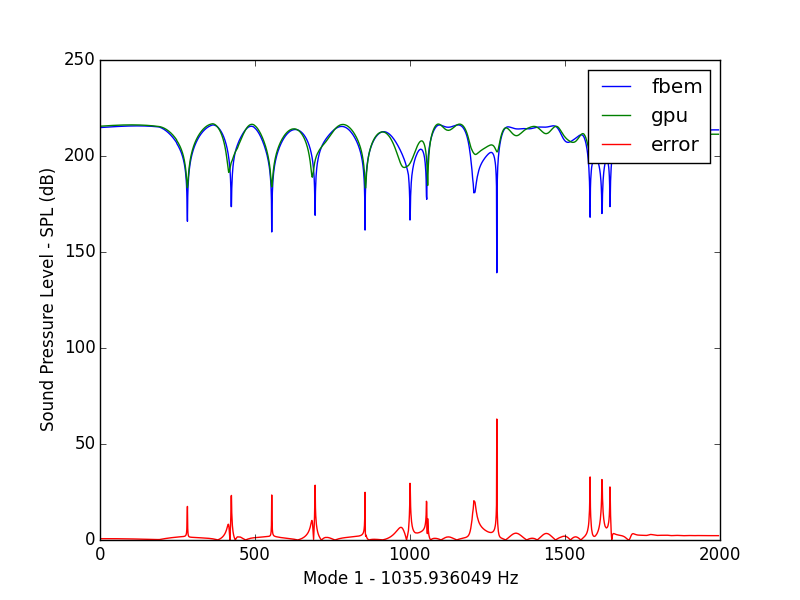
\includegraphics[width=\textwidth]{../data/transfer_test/ceramic_plate/plots/ceramic_plate-tfv-0_1.png}
	\caption{}
	\label{fig:coef_plate_1}
\end{subfigure}%
\begin{subfigure}{0.45\textwidth}
	\centering
	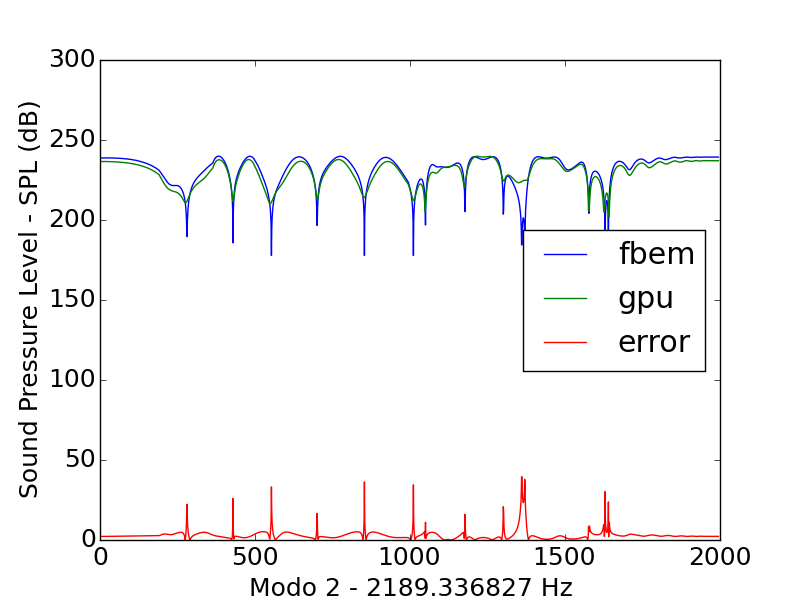
\includegraphics[width=\textwidth]{../data/transfer_test/ceramic_plate/plots/ceramic_plate-tfv-0_2.png}
	\label{fig:coef_plate_2}
	\caption{}
\end{subfigure}
\begin{subfigure}{0.45\textwidth}
	\centering
	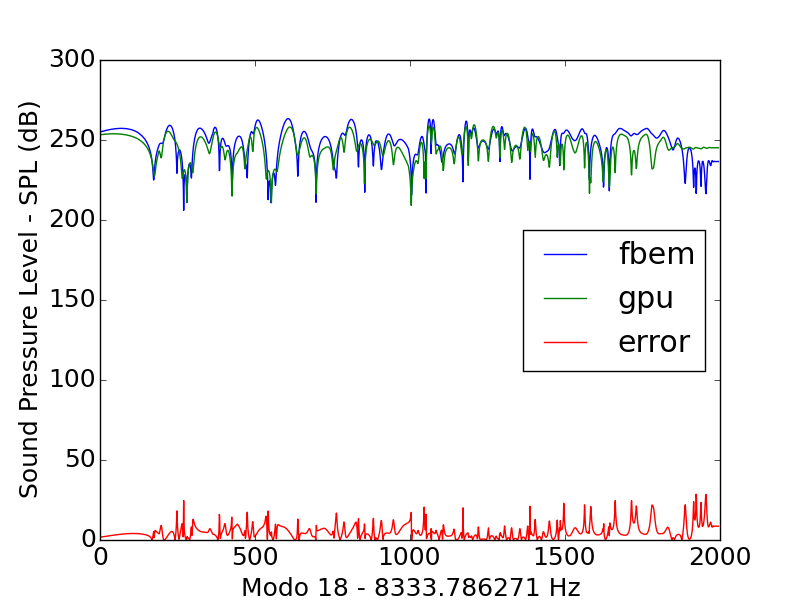
\includegraphics[width=\textwidth]{../data/transfer_test/ceramic_plate/plots/ceramic_plate-tfv-0_18.png}
	\caption{}
	\label{fig:coef_plate_18}
\end{subfigure}%
\begin{subfigure}{0.45\textwidth}
	\centering
	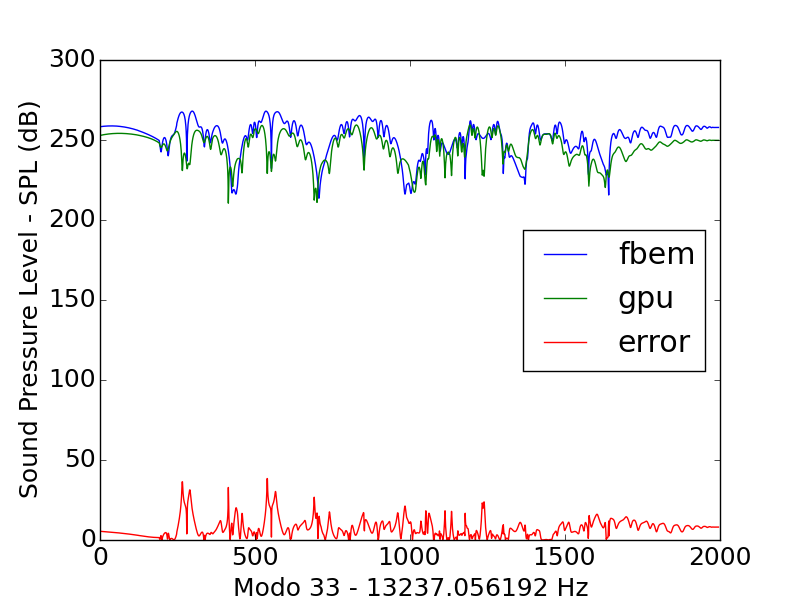
\includegraphics[width=\textwidth]{../data/transfer_test/ceramic_plate/plots/ceramic_plate-tfv-0_33.png}
	\caption{}
	\label{fig:coef_plate_33}
\end{subfigure}
\caption[Comparação numérica para o Prato de Cerâmica]{Comparação numérica para o Prato de Cerâmica. As figuras apresentam a comparação do módulo dos coeficientes para modos de vibração específicos.}
\label{fig:coef_plate}
\end{figure}

% \begin{figure}[ht] \label{fig:coef_mug_delta}
% \centering
% 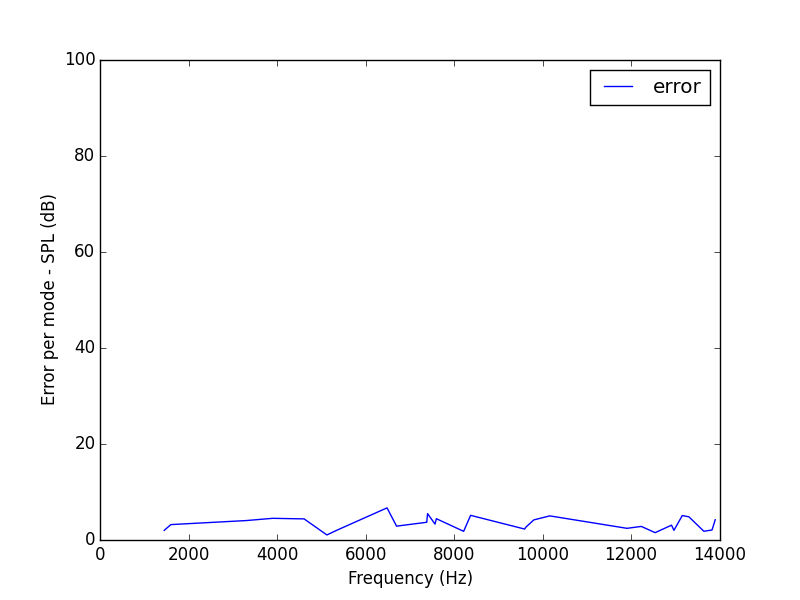
\includegraphics[width=0.6\textwidth]{../data/transfer_test/ceramic_mug/plots/ceramic_mug_error.png}
% \caption[Comparação numérica para a Caneca de Cerâmica]{Comparação numérica para a Caneca de Cerâmica. A figura ao topo apresenta o Erro Médio por frequência. As demais figuras apresentam a comparação para modos de vibração específicos.}
% \end{figure}

% \begin{figure}[ht] \label{fig:coef_key_delta}
% \centering
% 	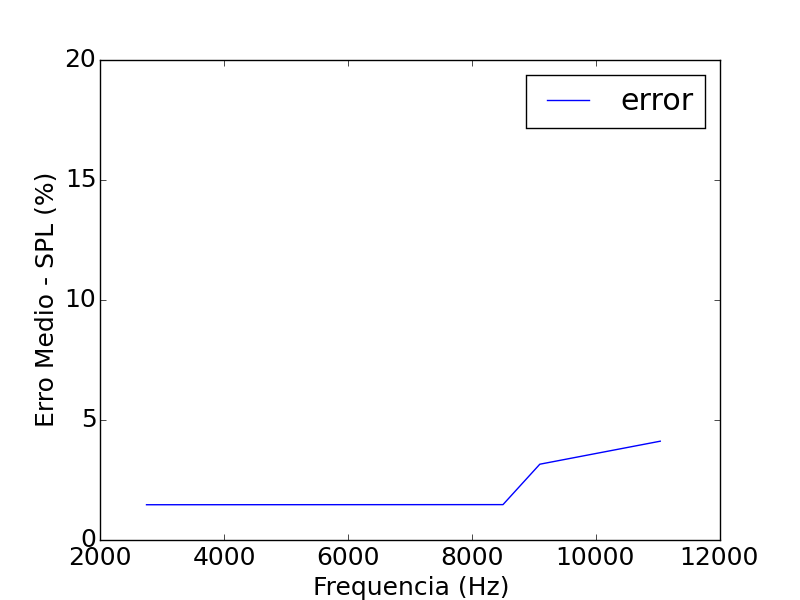
\includegraphics[width=0.6\textwidth]{../data/transfer_test/steel_key/plots/steel_key_error.png}
% \caption[Comparação numérica para a Chave de Aço]{Comparação numérica para a Chave de Aço. A figura ao topo apresenta o Erro Médio por frequência. As demais figuras apresentam a comparação para modos de vibração específicos.}
% \end{figure}

\begin{figure}[ht]
\centering
\begin{subfigure}{0.6\textwidth}
\centering
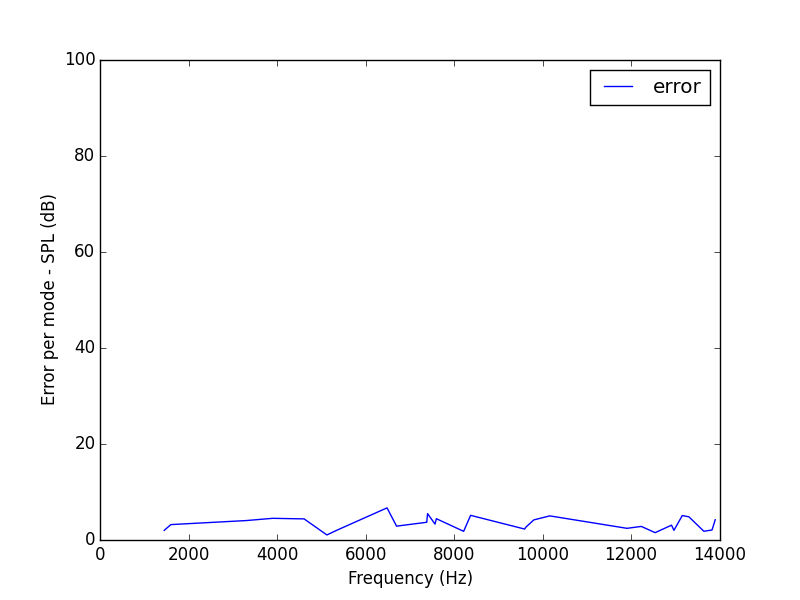
\includegraphics[width=\textwidth]{../data/transfer_test/ceramic_mug/plots/ceramic_mug_error.png}
\end{subfigure}
\begin{subfigure}{0.45\textwidth}
	\centering
	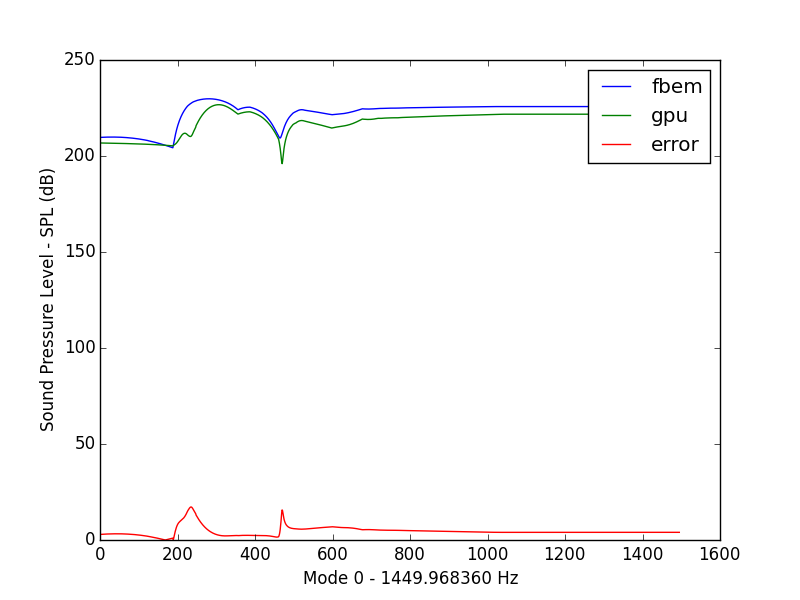
\includegraphics[width=\textwidth]{../data/transfer_test/ceramic_mug/plots/ceramic_mug-tfv-0_0.png}
	\caption{}
	\label{fig:coef_mug_0}
\end{subfigure}%
\begin{subfigure}{0.45\textwidth}
	\centering
	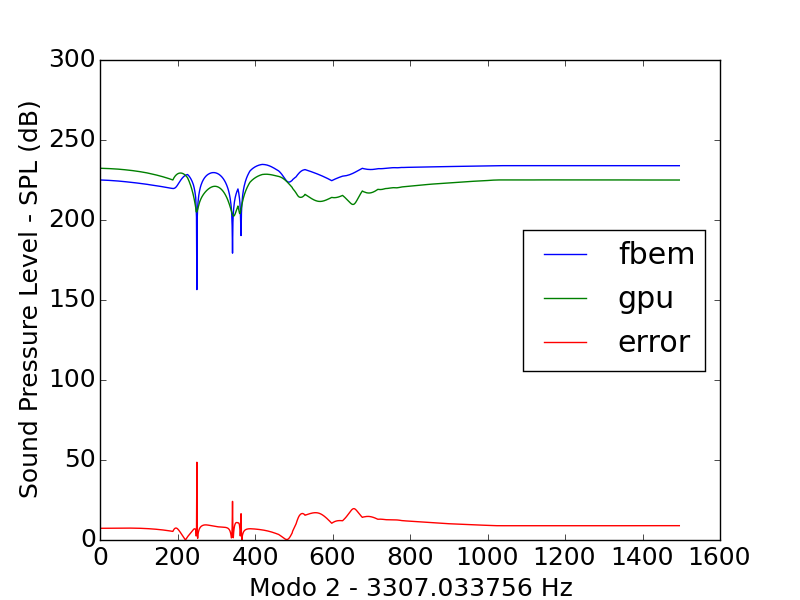
\includegraphics[width=\textwidth]{../data/transfer_test/ceramic_mug/plots/ceramic_mug-tfv-0_2.png}
	\caption{}
	\label{fig:coef_mug_2}
\end{subfigure}
\begin{subfigure}{0.45\textwidth}
	\centering
	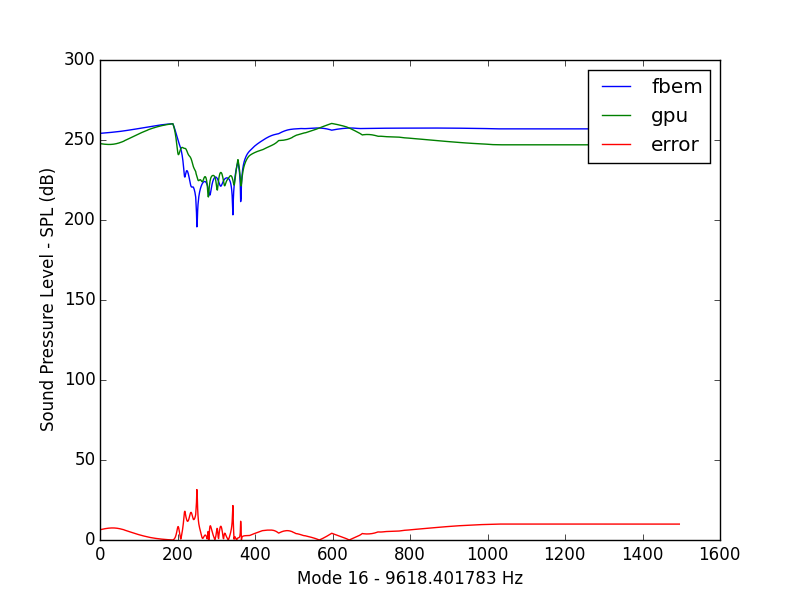
\includegraphics[width=\textwidth]{../data/transfer_test/ceramic_mug/plots/ceramic_mug-tfv-0_16.png}
	\caption{}
	\label{fig:coef_mug_16}
\end{subfigure}%
\begin{subfigure}{0.45\textwidth}
	\centering
	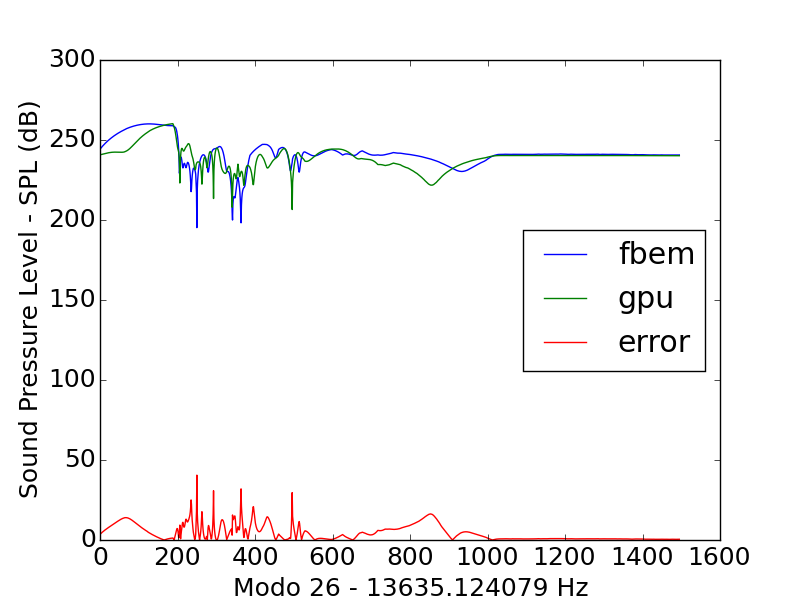
\includegraphics[width=\textwidth]{../data/transfer_test/ceramic_mug/plots/ceramic_mug-tfv-0_26.png}
	\caption{}
	\label{fig:coef_mug_26}
\end{subfigure}
\caption[Comparação numérica para a Caneca de Cerâmica]{Comparação numérica para a Caneca de Cerâmica. A figura ao topo apresenta a diferença numérica média por frequência. As demais figuras apresentam a comparação do módulo dos coeficientes para modos de vibração específicos.}
\label{fig:coef_mug_diff}
\end{figure}

\begin{figure}[ht]
\centering
\begin{subfigure}{0.6\textwidth}
\centering
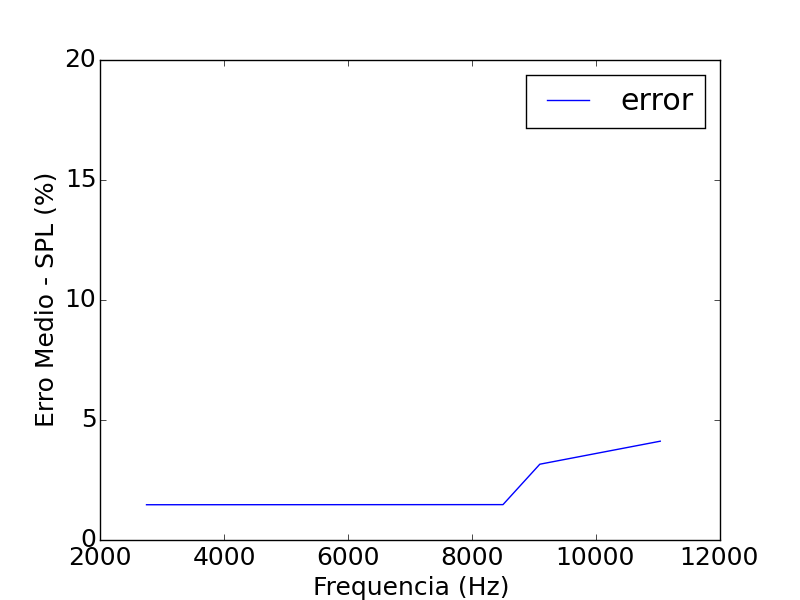
\includegraphics[width=\textwidth]{../data/transfer_test/steel_key/plots/steel_key_error.png}
\end{subfigure}
\begin{subfigure}{0.45\textwidth}
	\centering
	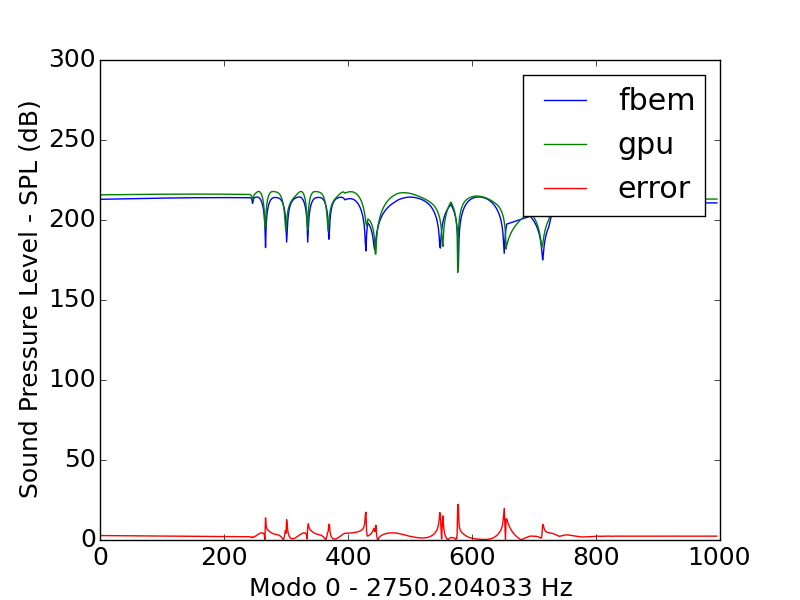
\includegraphics[width=\textwidth]{../data/transfer_test/steel_key/plots/steel_key-tfv-0_0.png}
	\caption{}
	\label{fig:coef_key_0}
\end{subfigure}%
\begin{subfigure}{0.45\textwidth}
	\centering
	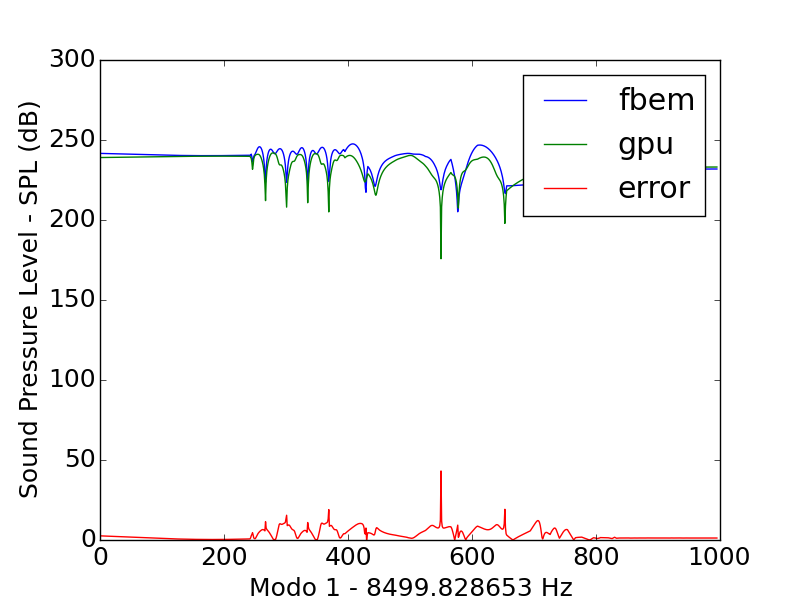
\includegraphics[width=\textwidth]{../data/transfer_test/steel_key/plots/steel_key-tfv-0_1.png}
	\caption{}
	\label{fig:coef_key_1}
\end{subfigure}
\begin{subfigure}{0.45\textwidth}
	\centering
	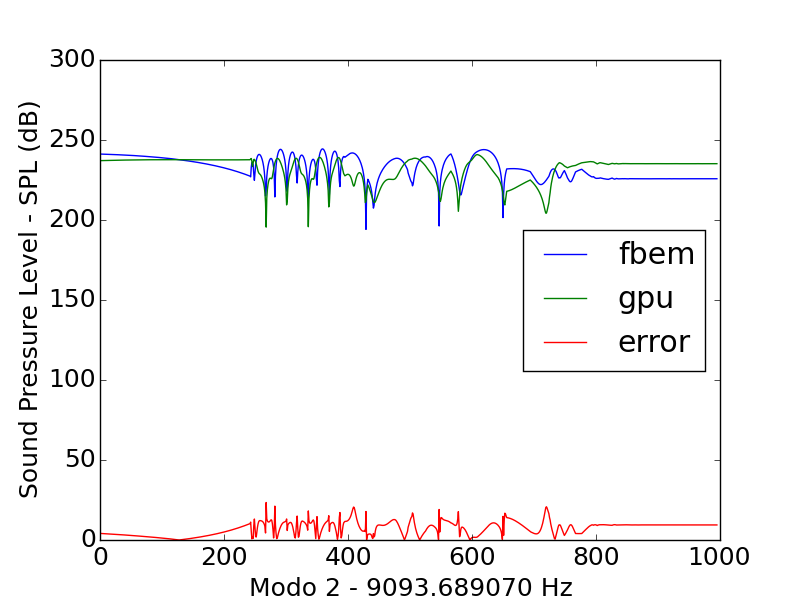
\includegraphics[width=\textwidth]{../data/transfer_test/steel_key/plots/steel_key-tfv-0_2.png}
	\caption{}
	\label{fig:coef_key_2}
\end{subfigure}%
\begin{subfigure}{0.45\textwidth}
	\centering
	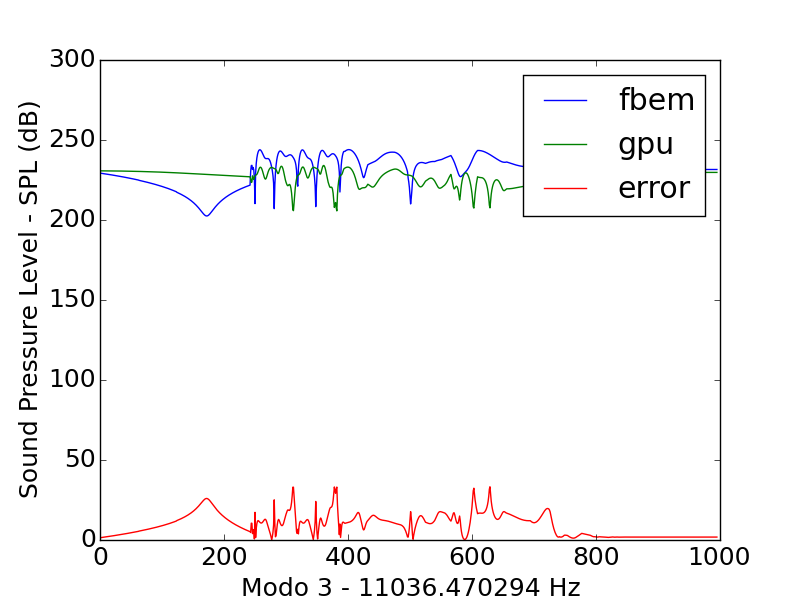
\includegraphics[width=\textwidth]{../data/transfer_test/steel_key/plots/steel_key-tfv-0_3.png}
	\caption{}
	\label{fig:coef_key_3}
\end{subfigure}
\caption[Comparação numérica para a Chave de Aço]{Comparação numérica para a Chave de Aço. A figura ao topo apresenta a diferença numérica média por frequência. As demais figuras apresentam a comparação do módulo dos coeficientes para modos de vibração específicos.}
\label{fig:coef_key_diff}
\end{figure}
% É aconselhável criar cada apêndice em um arquivo à parte, digamos
% "apendice1.tex", "apendice.tex", ... "apendiceM.tex" e depois
% incluí-los com:
% \include{apendice1}
% \include{apendice2}
% ...
% \include{apendiceM}


% Bibliografia
% É aconselhável utilizar o BibTeX a partir de um arquivo, digamos "biblio.bib".
% Para ajuda na criação do arquivo .bib e utilização do BibTeX, recorra ao
% BibTeXpress em www.cin.ufpe.br/~paguso/bibtexpress
%!TEX root = ../main.tex
\chapter{Algoritmo e Implementação}

\begin{figure}[ht]
\begin{subfigure}{\textwidth}
	\centering
	\input{algorithm/pipeline_offline.tikz}
	\caption[Pipeline off]{Sistema elastodinâmico unidimensional. Cada nó tem massa $m_i$ e cada mola tem uma constante $k_{i,j}$}\label{pipeline_offline}
\end{subfigure}
\begin{subfigure}{\textwidth}
	\centering
	\input{algorithm/pipeline_online.tikz}
	\caption[Pipeline on]{Sistema elastodinâmico unidimensional. Cada nó tem massa $m_i$ e cada mola tem uma constante $k_{i,j}$}\label{pipeline_online}
\end{subfigure}
\caption[Overview do pipeline]{\figref{pipeline_offline} plots of....}
\label{fig:pipeline_overview}
\end{figure}

\section {Decomposição Tetragonal}

\section {Simulação de Objetos Semi-rígidos}

\section {Aproximação da Equação de Helmholtz em GPU}

\section {Síntese}


% Cólofon
% Inclui uma pequena nota com referência à UFPEThesis
% Comente para omitir
% \colophon

%% Fim do documento
\end{document}
